% Created by tikzDevice version 0.12.4 on 2025-05-16 12:48:13
% !TEX encoding = UTF-8 Unicode
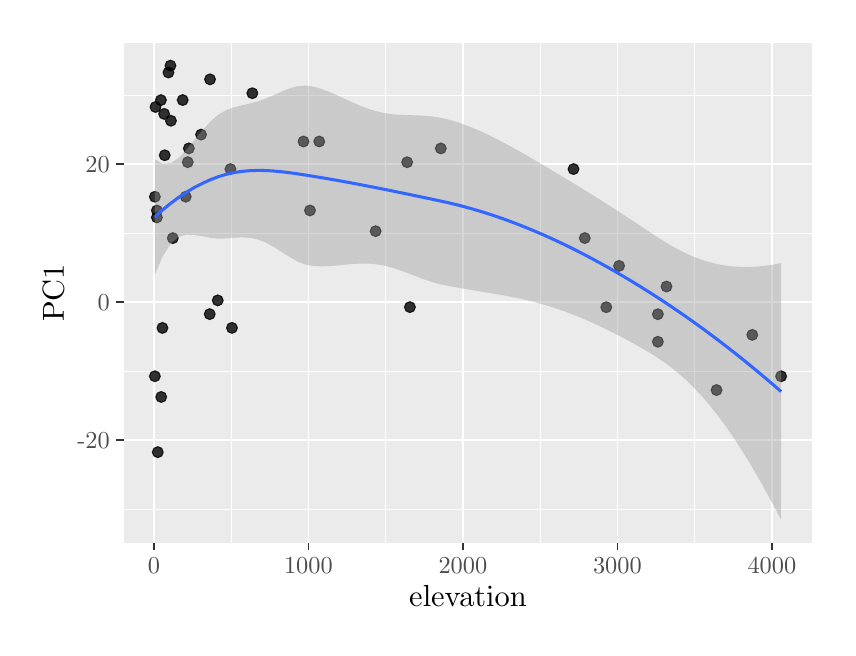
\begin{tikzpicture}[x=1pt,y=1pt]
\definecolor{fillColor}{RGB}{255,255,255}
\path[use as bounding box,fill=fillColor,fill opacity=0.00] (0,0) rectangle (289.08,216.81);
\begin{scope}
\path[clip] (  0.00,  0.00) rectangle (289.08,216.81);
\definecolor{drawColor}{RGB}{255,255,255}
\definecolor{fillColor}{RGB}{255,255,255}

\path[draw=drawColor,line width= 0.6pt,line join=round,line cap=round,fill=fillColor] (  0.00,  0.00) rectangle (289.08,216.81);
\end{scope}
\begin{scope}
\path[clip] ( 34.64, 30.69) rectangle (283.58,211.31);
\definecolor{fillColor}{gray}{0.92}

\path[fill=fillColor] ( 34.64, 30.69) rectangle (283.58,211.31);
\definecolor{drawColor}{RGB}{255,255,255}

\path[draw=drawColor,line width= 0.3pt,line join=round] ( 34.64, 42.76) --
	(283.58, 42.76);

\path[draw=drawColor,line width= 0.3pt,line join=round] ( 34.64, 92.63) --
	(283.58, 92.63);

\path[draw=drawColor,line width= 0.3pt,line join=round] ( 34.64,142.51) --
	(283.58,142.51);

\path[draw=drawColor,line width= 0.3pt,line join=round] ( 34.64,192.39) --
	(283.58,192.39);

\path[draw=drawColor,line width= 0.3pt,line join=round] ( 73.54, 30.69) --
	( 73.54,211.31);

\path[draw=drawColor,line width= 0.3pt,line join=round] (129.36, 30.69) --
	(129.36,211.31);

\path[draw=drawColor,line width= 0.3pt,line join=round] (185.18, 30.69) --
	(185.18,211.31);

\path[draw=drawColor,line width= 0.3pt,line join=round] (241.00, 30.69) --
	(241.00,211.31);

\path[draw=drawColor,line width= 0.6pt,line join=round] ( 34.64, 67.70) --
	(283.58, 67.70);

\path[draw=drawColor,line width= 0.6pt,line join=round] ( 34.64,117.57) --
	(283.58,117.57);

\path[draw=drawColor,line width= 0.6pt,line join=round] ( 34.64,167.45) --
	(283.58,167.45);

\path[draw=drawColor,line width= 0.6pt,line join=round] ( 45.63, 30.69) --
	( 45.63,211.31);

\path[draw=drawColor,line width= 0.6pt,line join=round] (101.45, 30.69) --
	(101.45,211.31);

\path[draw=drawColor,line width= 0.6pt,line join=round] (157.27, 30.69) --
	(157.27,211.31);

\path[draw=drawColor,line width= 0.6pt,line join=round] (213.09, 30.69) --
	(213.09,211.31);

\path[draw=drawColor,line width= 0.6pt,line join=round] (268.92, 30.69) --
	(268.92,211.31);
\definecolor{drawColor}{RGB}{0,0,0}
\definecolor{fillColor}{RGB}{0,0,0}

\path[draw=drawColor,draw opacity=0.80,line width= 0.4pt,line join=round,line cap=round,fill=fillColor,fill opacity=0.80] ( 48.14,190.63) circle (  1.96);

\path[draw=drawColor,draw opacity=0.80,line width= 0.4pt,line join=round,line cap=round,fill=fillColor,fill opacity=0.80] ( 51.60,203.10) circle (  1.96);

\path[draw=drawColor,draw opacity=0.80,line width= 0.4pt,line join=round,line cap=round,fill=fillColor,fill opacity=0.80] ( 46.18,188.14) circle (  1.96);

\path[draw=drawColor,draw opacity=0.80,line width= 0.4pt,line join=round,line cap=round,fill=fillColor,fill opacity=0.80] (230.84,123.26) circle (  1.96);

\path[draw=drawColor,draw opacity=0.80,line width= 0.4pt,line join=round,line cap=round,fill=fillColor,fill opacity=0.80] ( 45.96,155.70) circle (  1.96);

\path[draw=drawColor,draw opacity=0.80,line width= 0.4pt,line join=round,line cap=round,fill=fillColor,fill opacity=0.80] (102.01,150.76) circle (  1.96);

\path[draw=drawColor,draw opacity=0.80,line width= 0.4pt,line join=round,line cap=round,fill=fillColor,fill opacity=0.80] (209.07,115.79) circle (  1.96);

\path[draw=drawColor,draw opacity=0.80,line width= 0.4pt,line join=round,line cap=round,fill=fillColor,fill opacity=0.80] (201.31,140.78) circle (  1.96);

\path[draw=drawColor,draw opacity=0.80,line width= 0.4pt,line join=round,line cap=round,fill=fillColor,fill opacity=0.80] (149.29,173.18) circle (  1.96);

\path[draw=drawColor,draw opacity=0.80,line width= 0.4pt,line join=round,line cap=round,fill=fillColor,fill opacity=0.80] ( 51.77,183.17) circle (  1.96);

\path[draw=drawColor,draw opacity=0.80,line width= 0.4pt,line join=round,line cap=round,fill=fillColor,fill opacity=0.80] (272.26, 90.85) circle (  1.96);

\path[draw=drawColor,draw opacity=0.80,line width= 0.4pt,line join=round,line cap=round,fill=fillColor,fill opacity=0.80] ( 47.02, 63.43) circle (  1.96);

\path[draw=drawColor,draw opacity=0.80,line width= 0.4pt,line join=round,line cap=round,fill=fillColor,fill opacity=0.80] ( 68.68,118.27) circle (  1.96);

\path[draw=drawColor,draw opacity=0.80,line width= 0.4pt,line join=round,line cap=round,fill=fillColor,fill opacity=0.80] ( 58.24,173.19) circle (  1.96);

\path[draw=drawColor,draw opacity=0.80,line width= 0.4pt,line join=round,line cap=round,fill=fillColor,fill opacity=0.80] (248.93, 85.87) circle (  1.96);

\path[draw=drawColor,draw opacity=0.80,line width= 0.4pt,line join=round,line cap=round,fill=fillColor,fill opacity=0.80] (213.71,130.73) circle (  1.96);

\path[draw=drawColor,draw opacity=0.80,line width= 0.4pt,line join=round,line cap=round,fill=fillColor,fill opacity=0.80] (138.12,115.83) circle (  1.96);

\path[draw=drawColor,draw opacity=0.80,line width= 0.4pt,line join=round,line cap=round,fill=fillColor,fill opacity=0.80] ( 49.31,185.65) circle (  1.96);

\path[draw=drawColor,draw opacity=0.80,line width= 0.4pt,line join=round,line cap=round,fill=fillColor,fill opacity=0.80] ( 57.12,155.73) circle (  1.96);

\path[draw=drawColor,draw opacity=0.80,line width= 0.4pt,line join=round,line cap=round,fill=fillColor,fill opacity=0.80] ( 48.25, 83.37) circle (  1.96);

\path[draw=drawColor,draw opacity=0.80,line width= 0.4pt,line join=round,line cap=round,fill=fillColor,fill opacity=0.80] (197.24,165.72) circle (  1.96);

\path[draw=drawColor,draw opacity=0.80,line width= 0.4pt,line join=round,line cap=round,fill=fillColor,fill opacity=0.80] ( 99.66,175.68) circle (  1.96);

\path[draw=drawColor,draw opacity=0.80,line width= 0.4pt,line join=round,line cap=round,fill=fillColor,fill opacity=0.80] ( 65.78,113.30) circle (  1.96);

\path[draw=drawColor,draw opacity=0.80,line width= 0.4pt,line join=round,line cap=round,fill=fillColor,fill opacity=0.80] ( 81.18,193.13) circle (  1.96);

\path[draw=drawColor,draw opacity=0.80,line width= 0.4pt,line join=round,line cap=round,fill=fillColor,fill opacity=0.80] ( 65.89,198.13) circle (  1.96);

\path[draw=drawColor,draw opacity=0.80,line width= 0.4pt,line join=round,line cap=round,fill=fillColor,fill opacity=0.80] ( 73.26,165.71) circle (  1.96);

\path[draw=drawColor,draw opacity=0.80,line width= 0.4pt,line join=round,line cap=round,fill=fillColor,fill opacity=0.80] (137.12,168.19) circle (  1.96);

\path[draw=drawColor,draw opacity=0.80,line width= 0.4pt,line join=round,line cap=round,fill=fillColor,fill opacity=0.80] (105.36,175.68) circle (  1.96);

\path[draw=drawColor,draw opacity=0.80,line width= 0.4pt,line join=round,line cap=round,fill=fillColor,fill opacity=0.80] (125.73,143.27) circle (  1.96);

\path[draw=drawColor,draw opacity=0.80,line width= 0.4pt,line join=round,line cap=round,fill=fillColor,fill opacity=0.80] ( 57.85,168.21) circle (  1.96);

\path[draw=drawColor,draw opacity=0.80,line width= 0.4pt,line join=round,line cap=round,fill=fillColor,fill opacity=0.80] (227.72,113.27) circle (  1.96);

\path[draw=drawColor,draw opacity=0.80,line width= 0.4pt,line join=round,line cap=round,fill=fillColor,fill opacity=0.80] (227.72,103.31) circle (  1.96);

\path[draw=drawColor,draw opacity=0.80,line width= 0.4pt,line join=round,line cap=round,fill=fillColor,fill opacity=0.80] ( 62.65,178.17) circle (  1.96);

\path[draw=drawColor,draw opacity=0.80,line width= 0.4pt,line join=round,line cap=round,fill=fillColor,fill opacity=0.80] ( 50.87,200.61) circle (  1.96);

\path[draw=drawColor,draw opacity=0.80,line width= 0.4pt,line join=round,line cap=round,fill=fillColor,fill opacity=0.80] ( 45.96, 90.86) circle (  1.96);

\path[draw=drawColor,draw opacity=0.80,line width= 0.4pt,line join=round,line cap=round,fill=fillColor,fill opacity=0.80] ( 73.82,108.33) circle (  1.96);

\path[draw=drawColor,draw opacity=0.80,line width= 0.4pt,line join=round,line cap=round,fill=fillColor,fill opacity=0.80] ( 46.69,148.24) circle (  1.96);

\path[draw=drawColor,draw opacity=0.80,line width= 0.4pt,line join=round,line cap=round,fill=fillColor,fill opacity=0.80] ( 48.70,108.31) circle (  1.96);

\path[draw=drawColor,draw opacity=0.80,line width= 0.4pt,line join=round,line cap=round,fill=fillColor,fill opacity=0.80] ( 52.44,140.76) circle (  1.96);

\path[draw=drawColor,draw opacity=0.80,line width= 0.4pt,line join=round,line cap=round,fill=fillColor,fill opacity=0.80] ( 46.69,150.74) circle (  1.96);

\path[draw=drawColor,draw opacity=0.80,line width= 0.4pt,line join=round,line cap=round,fill=fillColor,fill opacity=0.80] (261.83,105.80) circle (  1.96);

\path[draw=drawColor,draw opacity=0.80,line width= 0.4pt,line join=round,line cap=round,fill=fillColor,fill opacity=0.80] ( 49.53,170.70) circle (  1.96);

\path[draw=drawColor,draw opacity=0.80,line width= 0.4pt,line join=round,line cap=round,fill=fillColor,fill opacity=0.80] ( 56.01,190.65) circle (  1.96);
\definecolor{fillColor}{RGB}{153,153,153}

\path[fill=fillColor,fill opacity=0.40] ( 45.96,169.21) --
	( 48.82,167.74) --
	( 51.69,167.87) --
	( 54.55,169.69) --
	( 57.42,172.76) --
	( 60.28,176.26) --
	( 63.15,179.67) --
	( 66.01,182.84) --
	( 68.88,185.35) --
	( 71.74,187.00) --
	( 74.61,188.04) --
	( 77.47,188.74) --
	( 80.34,189.40) --
	( 83.20,190.19) --
	( 86.06,191.22) --
	( 88.93,192.44) --
	( 91.79,193.71) --
	( 94.66,194.85) --
	( 97.52,195.64) --
	(100.39,195.89) --
	(103.25,195.48) --
	(106.12,194.67) --
	(108.98,193.61) --
	(111.85,192.38) --
	(114.71,191.05) --
	(117.58,189.73) --
	(120.44,188.50) --
	(123.30,187.42) --
	(126.17,186.56) --
	(129.03,185.93) --
	(131.90,185.52) --
	(134.76,185.30) --
	(137.63,185.19) --
	(140.49,185.12) --
	(143.36,184.99) --
	(146.22,184.74) --
	(149.09,184.29) --
	(151.95,183.63) --
	(154.82,182.80) --
	(157.68,181.83) --
	(160.54,180.73) --
	(163.41,179.51) --
	(166.27,178.18) --
	(169.14,176.76) --
	(172.00,175.27) --
	(174.87,173.72) --
	(177.73,172.12) --
	(180.60,170.48) --
	(183.46,168.81) --
	(186.33,167.12) --
	(189.19,165.41) --
	(192.06,163.70) --
	(194.92,161.97) --
	(197.78,160.24) --
	(200.65,158.49) --
	(203.51,156.72) --
	(206.38,154.94) --
	(209.24,153.13) --
	(212.11,151.30) --
	(214.97,149.44) --
	(217.84,147.55) --
	(220.70,145.65) --
	(223.57,143.74) --
	(226.43,141.85) --
	(229.30,140.01) --
	(232.16,138.28) --
	(235.02,136.69) --
	(237.89,135.25) --
	(240.75,133.99) --
	(243.62,132.92) --
	(246.48,132.04) --
	(249.35,131.35) --
	(252.21,130.85) --
	(255.08,130.52) --
	(257.94,130.36) --
	(260.81,130.35) --
	(263.67,130.50) --
	(266.54,130.78) --
	(269.40,131.19) --
	(272.26,131.72) --
	(272.26, 38.90) --
	(269.40, 44.39) --
	(266.54, 49.69) --
	(263.67, 54.77) --
	(260.81, 59.63) --
	(257.94, 64.27) --
	(255.08, 68.66) --
	(252.21, 72.80) --
	(249.35, 76.68) --
	(246.48, 80.29) --
	(243.62, 83.64) --
	(240.75, 86.70) --
	(237.89, 89.50) --
	(235.02, 92.04) --
	(232.16, 94.33) --
	(229.30, 96.40) --
	(226.43, 98.29) --
	(223.57,100.04) --
	(220.70,101.70) --
	(217.84,103.30) --
	(214.97,104.83) --
	(212.11,106.31) --
	(209.24,107.73) --
	(206.38,109.10) --
	(203.51,110.42) --
	(200.65,111.67) --
	(197.78,112.84) --
	(194.92,113.95) --
	(192.06,114.98) --
	(189.19,115.92) --
	(186.33,116.79) --
	(183.46,117.58) --
	(180.60,118.29) --
	(177.73,118.94) --
	(174.87,119.53) --
	(172.00,120.07) --
	(169.14,120.57) --
	(166.27,121.05) --
	(163.41,121.51) --
	(160.54,121.98) --
	(157.68,122.46) --
	(154.82,122.96) --
	(151.95,123.50) --
	(149.09,124.10) --
	(146.22,124.86) --
	(143.36,125.81) --
	(140.49,126.89) --
	(137.63,128.01) --
	(134.76,129.08) --
	(131.90,130.03) --
	(129.03,130.78) --
	(126.17,131.29) --
	(123.30,131.55) --
	(120.44,131.58) --
	(117.58,131.43) --
	(114.71,131.17) --
	(111.85,130.88) --
	(108.98,130.65) --
	(106.12,130.57) --
	(103.25,130.71) --
	(100.39,131.21) --
	( 97.52,132.33) --
	( 94.66,133.93) --
	( 91.79,135.76) --
	( 88.93,137.58) --
	( 86.06,139.14) --
	( 83.20,140.27) --
	( 80.34,140.88) --
	( 77.47,141.03) --
	( 74.61,140.88) --
	( 71.74,140.64) --
	( 68.88,140.57) --
	( 66.01,140.88) --
	( 63.15,141.43) --
	( 60.28,141.90) --
	( 57.42,142.01) --
	( 54.55,141.24) --
	( 51.69,138.83) --
	( 48.82,134.25) --
	( 45.96,127.56) --
	cycle;

\path[] ( 45.96,169.21) --
	( 48.82,167.74) --
	( 51.69,167.87) --
	( 54.55,169.69) --
	( 57.42,172.76) --
	( 60.28,176.26) --
	( 63.15,179.67) --
	( 66.01,182.84) --
	( 68.88,185.35) --
	( 71.74,187.00) --
	( 74.61,188.04) --
	( 77.47,188.74) --
	( 80.34,189.40) --
	( 83.20,190.19) --
	( 86.06,191.22) --
	( 88.93,192.44) --
	( 91.79,193.71) --
	( 94.66,194.85) --
	( 97.52,195.64) --
	(100.39,195.89) --
	(103.25,195.48) --
	(106.12,194.67) --
	(108.98,193.61) --
	(111.85,192.38) --
	(114.71,191.05) --
	(117.58,189.73) --
	(120.44,188.50) --
	(123.30,187.42) --
	(126.17,186.56) --
	(129.03,185.93) --
	(131.90,185.52) --
	(134.76,185.30) --
	(137.63,185.19) --
	(140.49,185.12) --
	(143.36,184.99) --
	(146.22,184.74) --
	(149.09,184.29) --
	(151.95,183.63) --
	(154.82,182.80) --
	(157.68,181.83) --
	(160.54,180.73) --
	(163.41,179.51) --
	(166.27,178.18) --
	(169.14,176.76) --
	(172.00,175.27) --
	(174.87,173.72) --
	(177.73,172.12) --
	(180.60,170.48) --
	(183.46,168.81) --
	(186.33,167.12) --
	(189.19,165.41) --
	(192.06,163.70) --
	(194.92,161.97) --
	(197.78,160.24) --
	(200.65,158.49) --
	(203.51,156.72) --
	(206.38,154.94) --
	(209.24,153.13) --
	(212.11,151.30) --
	(214.97,149.44) --
	(217.84,147.55) --
	(220.70,145.65) --
	(223.57,143.74) --
	(226.43,141.85) --
	(229.30,140.01) --
	(232.16,138.28) --
	(235.02,136.69) --
	(237.89,135.25) --
	(240.75,133.99) --
	(243.62,132.92) --
	(246.48,132.04) --
	(249.35,131.35) --
	(252.21,130.85) --
	(255.08,130.52) --
	(257.94,130.36) --
	(260.81,130.35) --
	(263.67,130.50) --
	(266.54,130.78) --
	(269.40,131.19) --
	(272.26,131.72);

\path[] (272.26, 38.90) --
	(269.40, 44.39) --
	(266.54, 49.69) --
	(263.67, 54.77) --
	(260.81, 59.63) --
	(257.94, 64.27) --
	(255.08, 68.66) --
	(252.21, 72.80) --
	(249.35, 76.68) --
	(246.48, 80.29) --
	(243.62, 83.64) --
	(240.75, 86.70) --
	(237.89, 89.50) --
	(235.02, 92.04) --
	(232.16, 94.33) --
	(229.30, 96.40) --
	(226.43, 98.29) --
	(223.57,100.04) --
	(220.70,101.70) --
	(217.84,103.30) --
	(214.97,104.83) --
	(212.11,106.31) --
	(209.24,107.73) --
	(206.38,109.10) --
	(203.51,110.42) --
	(200.65,111.67) --
	(197.78,112.84) --
	(194.92,113.95) --
	(192.06,114.98) --
	(189.19,115.92) --
	(186.33,116.79) --
	(183.46,117.58) --
	(180.60,118.29) --
	(177.73,118.94) --
	(174.87,119.53) --
	(172.00,120.07) --
	(169.14,120.57) --
	(166.27,121.05) --
	(163.41,121.51) --
	(160.54,121.98) --
	(157.68,122.46) --
	(154.82,122.96) --
	(151.95,123.50) --
	(149.09,124.10) --
	(146.22,124.86) --
	(143.36,125.81) --
	(140.49,126.89) --
	(137.63,128.01) --
	(134.76,129.08) --
	(131.90,130.03) --
	(129.03,130.78) --
	(126.17,131.29) --
	(123.30,131.55) --
	(120.44,131.58) --
	(117.58,131.43) --
	(114.71,131.17) --
	(111.85,130.88) --
	(108.98,130.65) --
	(106.12,130.57) --
	(103.25,130.71) --
	(100.39,131.21) --
	( 97.52,132.33) --
	( 94.66,133.93) --
	( 91.79,135.76) --
	( 88.93,137.58) --
	( 86.06,139.14) --
	( 83.20,140.27) --
	( 80.34,140.88) --
	( 77.47,141.03) --
	( 74.61,140.88) --
	( 71.74,140.64) --
	( 68.88,140.57) --
	( 66.01,140.88) --
	( 63.15,141.43) --
	( 60.28,141.90) --
	( 57.42,142.01) --
	( 54.55,141.24) --
	( 51.69,138.83) --
	( 48.82,134.25) --
	( 45.96,127.56);
\definecolor{drawColor}{RGB}{51,102,255}

\path[draw=drawColor,line width= 1.1pt,line join=round] ( 45.96,148.39) --
	( 48.82,151.00) --
	( 51.69,153.35) --
	( 54.55,155.46) --
	( 57.42,157.38) --
	( 60.28,159.08) --
	( 63.15,160.55) --
	( 66.01,161.86) --
	( 68.88,162.96) --
	( 71.74,163.82) --
	( 74.61,164.46) --
	( 77.47,164.89) --
	( 80.34,165.14) --
	( 83.20,165.23) --
	( 86.06,165.18) --
	( 88.93,165.01) --
	( 91.79,164.74) --
	( 94.66,164.39) --
	( 97.52,163.99) --
	(100.39,163.55) --
	(103.25,163.09) --
	(106.12,162.62) --
	(108.98,162.13) --
	(111.85,161.63) --
	(114.71,161.11) --
	(117.58,160.58) --
	(120.44,160.04) --
	(123.30,159.49) --
	(126.17,158.93) --
	(129.03,158.35) --
	(131.90,157.78) --
	(134.76,157.19) --
	(137.63,156.60) --
	(140.49,156.00) --
	(143.36,155.40) --
	(146.22,154.80) --
	(149.09,154.19) --
	(151.95,153.56) --
	(154.82,152.88) --
	(157.68,152.14) --
	(160.54,151.35) --
	(163.41,150.51) --
	(166.27,149.61) --
	(169.14,148.67) --
	(172.00,147.67) --
	(174.87,146.62) --
	(177.73,145.53) --
	(180.60,144.38) --
	(183.46,143.19) --
	(186.33,141.95) --
	(189.19,140.67) --
	(192.06,139.34) --
	(194.92,137.96) --
	(197.78,136.54) --
	(200.65,135.08) --
	(203.51,133.57) --
	(206.38,132.02) --
	(209.24,130.43) --
	(212.11,128.80) --
	(214.97,127.13) --
	(217.84,125.42) --
	(220.70,123.67) --
	(223.57,121.89) --
	(226.43,120.07) --
	(229.30,118.21) --
	(232.16,116.30) --
	(235.02,114.36) --
	(237.89,112.38) --
	(240.75,110.35) --
	(243.62,108.28) --
	(246.48,106.17) --
	(249.35,104.02) --
	(252.21,101.82) --
	(255.08, 99.59) --
	(257.94, 97.31) --
	(260.81, 94.99) --
	(263.67, 92.63) --
	(266.54, 90.23) --
	(269.40, 87.79) --
	(272.26, 85.31);
\end{scope}
\begin{scope}
\path[clip] (  0.00,  0.00) rectangle (289.08,216.81);
\definecolor{drawColor}{gray}{0.30}

\node[text=drawColor,anchor=base east,inner sep=0pt, outer sep=0pt, scale=  0.88] at ( 29.69, 64.67) {-20};

\node[text=drawColor,anchor=base east,inner sep=0pt, outer sep=0pt, scale=  0.88] at ( 29.69,114.54) {0};

\node[text=drawColor,anchor=base east,inner sep=0pt, outer sep=0pt, scale=  0.88] at ( 29.69,164.42) {20};
\end{scope}
\begin{scope}
\path[clip] (  0.00,  0.00) rectangle (289.08,216.81);
\definecolor{drawColor}{gray}{0.20}

\path[draw=drawColor,line width= 0.6pt,line join=round] ( 31.89, 67.70) --
	( 34.64, 67.70);

\path[draw=drawColor,line width= 0.6pt,line join=round] ( 31.89,117.57) --
	( 34.64,117.57);

\path[draw=drawColor,line width= 0.6pt,line join=round] ( 31.89,167.45) --
	( 34.64,167.45);
\end{scope}
\begin{scope}
\path[clip] (  0.00,  0.00) rectangle (289.08,216.81);
\definecolor{drawColor}{gray}{0.20}

\path[draw=drawColor,line width= 0.6pt,line join=round] ( 45.63, 27.94) --
	( 45.63, 30.69);

\path[draw=drawColor,line width= 0.6pt,line join=round] (101.45, 27.94) --
	(101.45, 30.69);

\path[draw=drawColor,line width= 0.6pt,line join=round] (157.27, 27.94) --
	(157.27, 30.69);

\path[draw=drawColor,line width= 0.6pt,line join=round] (213.09, 27.94) --
	(213.09, 30.69);

\path[draw=drawColor,line width= 0.6pt,line join=round] (268.92, 27.94) --
	(268.92, 30.69);
\end{scope}
\begin{scope}
\path[clip] (  0.00,  0.00) rectangle (289.08,216.81);
\definecolor{drawColor}{gray}{0.30}

\node[text=drawColor,anchor=base,inner sep=0pt, outer sep=0pt, scale=  0.88] at ( 45.63, 19.68) {0};

\node[text=drawColor,anchor=base,inner sep=0pt, outer sep=0pt, scale=  0.88] at (101.45, 19.68) {1000};

\node[text=drawColor,anchor=base,inner sep=0pt, outer sep=0pt, scale=  0.88] at (157.27, 19.68) {2000};

\node[text=drawColor,anchor=base,inner sep=0pt, outer sep=0pt, scale=  0.88] at (213.09, 19.68) {3000};

\node[text=drawColor,anchor=base,inner sep=0pt, outer sep=0pt, scale=  0.88] at (268.92, 19.68) {4000};
\end{scope}
\begin{scope}
\path[clip] (  0.00,  0.00) rectangle (289.08,216.81);
\definecolor{drawColor}{RGB}{0,0,0}

\node[text=drawColor,anchor=base,inner sep=0pt, outer sep=0pt, scale=  1.10] at (159.11,  7.64) {elevation};
\end{scope}
\begin{scope}
\path[clip] (  0.00,  0.00) rectangle (289.08,216.81);
\definecolor{drawColor}{RGB}{0,0,0}

\node[text=drawColor,rotate= 90.00,anchor=base,inner sep=0pt, outer sep=0pt, scale=  1.10] at ( 13.08,121.00) {PC1};
\end{scope}
\end{tikzpicture}
